\begin{frame}{Why Even Bother With Packaging?}
  \begin{center}
    \huge\textcolor{ccyan!90!cblack}{\textbf{Packages allow you to share your code, so other people can use it.}}
  \end{center}
  \vspace{2em}
  \textcolor{cpink}{But also\dots}
  \begin{itemize}
    \setlength{\itemsep}{1em}
    \item Helps you keeping your code from breaking
    \item Benefits other people that may have faced a similar problem
    \item Saves time because code can be reused easily
  \end{itemize}
\end{frame}

\begin{frame}{Before We Start: Package and Environment Managers}
  \begin{description}
    \setlength{\itemsep}{1em}
    \item [\iref{https://pypi.org/project/pip/}{pip}] The standard package installer for Python. \texttt{pip} is able to install
      directly from PyPI and other indexes.
    \item [\iref{https://mamba.readthedocs.io/en/latest/}{mamba}] Fast and robust, with cross-platform support. Written in \cpp.
      Allows you to manage multiple, isolated environments. \texttt{mamba} installs from local or remote package repositories, \eg, channels.
    \item [\iref{https://python-poetry.org/}{poetry}] Package installer that is also able to create its own virtual environments.
      Handles dependency resolving better than pip. Works nicely with \texttt{pyproject.toml} files. Allows the use of lock files.
    \item [\iref{https://docs.astral.sh/uv/}{uv}] A new and fast package manager written in {\footnotesize{\faRust}}\,\texttt{Rust}. Can create
      virtual environments, and solves dependencies better and faster than pip. Allows the use of lock files.
  \end{description}
  \begin{center}
    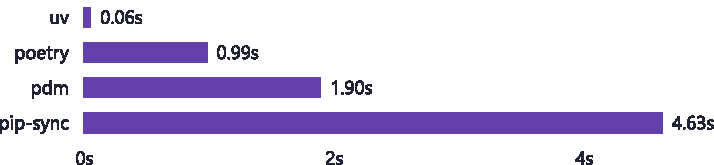
\includegraphics[width=0.7\textwidth]{graphics/speed.pdf}
    \src{docs.astral.sh/uv}
  \end{center}
\end{frame}




